\chapter{Research}
\section{Proposed System}
We are developing a smart helmet using the internet of things (IoT) technology, in which we ensure the safety of the bike rider. by avoiding road accidents of the bikers by following ways:
\begin{itemize}
	\item The system detects whether the rider is wearing a helmet or not if he wears then only the vehicle will start.
	
	\item It detects the amount of alcohol consumed by the rider, if the rider has over drunk, the bike engine will not start.
	
	\item When the bike rider meets with an accident it detects it and gives the notification to the registered contact with a location.
	
\end{itemize}
For the safety of the bike rider, we are using the latest technology IoT, this technology provides the advance techniques for alerting the rider and ensures that rider follows the rules and regulations. For two-wheeler rider, Helmet is the most basic protection device and it is necessary for every bicycle or motorbike riders. But it does not ensure the safety of the rider and the rider wont follow the traffic rules. Most of the people use ordinary helmet just to avoid giving challan to the traffic police, these helmets do not ensure the safety of the driver. So, to overcome these problems we need to use the smart helmet.

\begin{figure}[h]
	\centering
	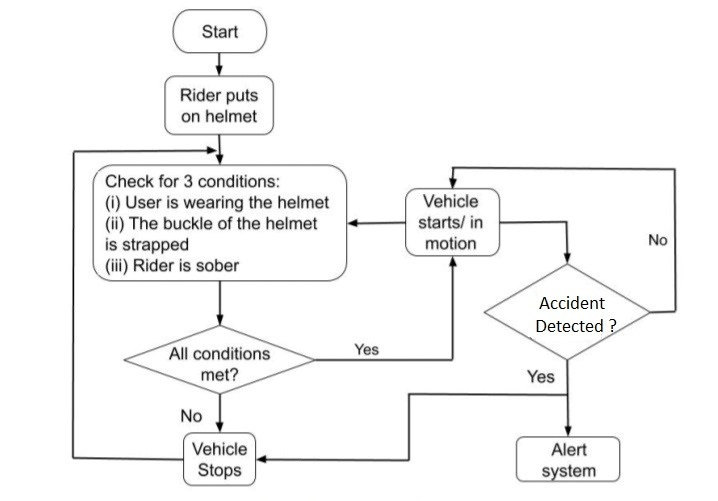
\includegraphics[scale=.55]{Flow diagram of the system.jpg}
	\caption{Flow diagram of the proposed system.}
\end{figure}
\pagebreak
\section{System Design}
Systems design is the process of defining elements of a system like modules, architecture, components and their interfaces and data for a system based on the specified requirements. It is the process of defining, developing and designing systems which satisfies the specific needs and requirements of a business or organization.
\vspace{.5cm}

In this case our system is smart helmet and this system has two sections namely,
\begin{itemize}
	\item Helmet section
	
	\item Bike section	
\end{itemize}
\section{Helmet Section}
The Helmet Unit consists of different sensors which collect the required information from the surrounding and then send it to the microcontroller for processing.
\vspace{.5cm}

\begin{figure}[h]
	\centering
	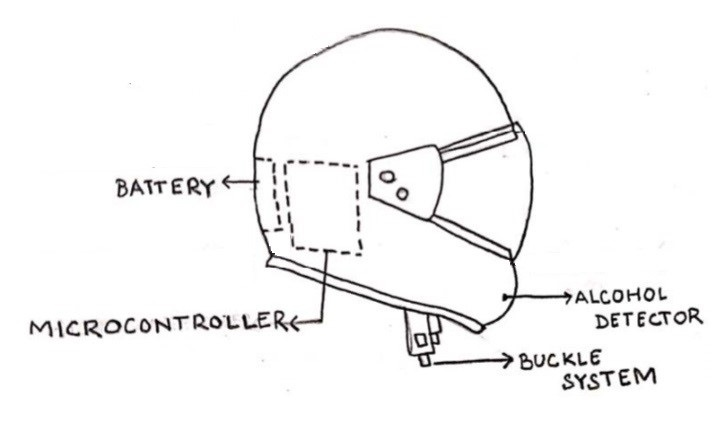
\includegraphics[scale=.9]{helmet unit.jpg}
	\caption{Helmet unit.}
\end{figure}

The Helmet Unit is battery-powered. Battery supplies the power to the whole circuit.
\begin{itemize}
	
	\item The buckle is used to secure the helmet on the head of the rider in order to protect him from the accident. The buckle system uses a Single Pole Double Throw switch to provide the guarantee that the buckle is effectively clasped before the riding of the two-wheeler by the rider.
	
	\item The alcohol detector is a Gas Sensor for the detection of the presence of alcohol in the rider’s breath and for determining his sobriety. An appropriate threshold value is set according to the laws of road safety. 
	
	\item The microcontroller section is where the microcontroller is encased. The microcontroller is used for capturing the signals from presence detector and alcohol detector. It processes the data and then generates a desirable output. This output is then sent to the vehicle unit for further functionality.
	
	\item Then the analysis of combined outputs from all the subsystems and sensors is done. Depending on the three primary conditions which needs to be checked, the microcontroller then generates a Boolean value. That value is transmitted over to the Vehicle Unit.
\end{itemize}
\pagebreak

\textbf{	The elements in Fig  are explained as follows:}

\subsection{MQ3 Alcohol Sensor}
MQ3 is one of the most commonly used sensors in the MQ sensor series. It is a Metal Oxide Semiconductor (MOS) type of sensor. Metal oxide sensors are also known as Chemiresistors, because sensing is based on the change of resistance of the sensing material when exposed to alcohol. So by placing it in a simple voltage divider network, alcohol concentrations can be detected.
\vspace{.5cm}

\begin{figure}[h]
	\centering
	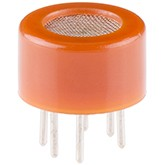
\includegraphics[scale=.55]{MQ3-Alcohol-Sensor.jpg}
	\caption{MQ3-Alcohol-Sensor}
\end{figure}

MQ3 alcohol sensor works on 5V DC and draws around 800mW. It can detect Alcohol concentrations anywhere from 25 to 500 ppm.

\begin{table}[h]
	\begin{center}
		
		%\label{Table 1.1}
		\begin{tabular}{l|l} 
			\textbf{Factor} & \textbf{Value} \\
			\hline
			\textbf{Operating voltage} & 5V\%\\
			\textbf{Load resistance}	& 200 K Ohm\\
			\textbf{Heater resistance} &	33 Ohm ± 5\%\\
			\textbf{Heating consumption}	& Less than 800mw\\
			\textbf{Sensing Resistance}	& 1 M Ohm – 8 M Ohm\\
			\textbf{Concentration Scope}	& 25 – 500 ppm\\
			\textbf{Preheat Time}	& Over 24 hour
			
		\end{tabular}\caption{Here are the complete specifications of MQ3 Alcohol Sensor.}
	\end{center}
\end{table}

\subsection{Internal structure of MQ3 Alcohol Sensor}
MQ3 is a heater-driven sensor. That’s why it is enclosed in two layers of fine stainless steel mesh called an Anti-explosion network. It ensures that heater element inside the sensor will not cause an explosion, as we are sensing flammable gas (alcohol).

\begin{figure}[h]
	\centering
	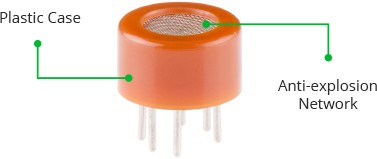
\includegraphics[scale=1.5]{MQ3-Alcohol-Sensor-Parts-Hardware-Overview.jpg}
	\caption{MQ3 Alcohol Sensor Upper Section.}
\end{figure}
It also provides protection for the sensor and filters out suspended particles so that only gaseous elements are able to pass inside the chamber.
\pagebreak
\begin{figure}[h]
	\centering
	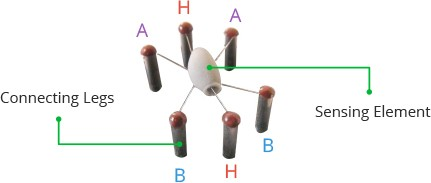
\includegraphics[scale=.4]{MQ3-Alcohol-Sensor-Internal-Structure.jpg}
	\caption{MQ3 Alcohol Sensor Pin Section.}
\end{figure}

\subsection{How MQ3 Alcohol Sensor Works?}
When SnO2 semiconductor layer is heated at high temperature, oxygen is adsorbed on the surface. In clean air, electrons from the conduction band in tin dioxide are attracted to oxygen molecules. This form an electron depletion layer just below the surface of SnO2 particles and forms a potential barrier. As a result, the SnO2 film becomes highly resistive and prevents electric current flow.

In the presence of alcohol, however, the surface density of adsorbed oxygen decreases as it reacts with the alcohols; which lowers the potential barrier. Electrons are then released into the tin dioxide, allowing current to flow freely through the sensor.

\begin{figure}[h]
	\centering
	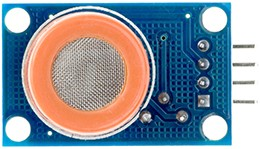
\includegraphics[scale=.6]{MQ3-Alcohol-Sensor-Module.jpg}
	\caption{MQ3 Alcohol Sensor.}
\end{figure}
\subsection{MQ3 Alcohol Sensor Module Pinout}
Now let’s have a look at the pinout.
\begin{figure}[h]
	\centering
	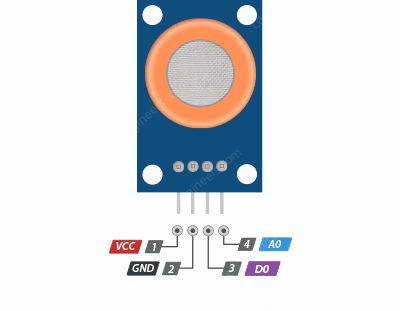
\includegraphics[scale=.7]{MQ3-Alcohol-Sensor-Pinout.png}
	\caption{MQ3 Alcohol Sensor Pin Diagram.}
\end{figure}

\textbf{VCC} supplies power for the module. You can connect it to 5V output from your Arduino.

\textbf{GND }is the Ground Pin and needs to be connected to GND pin on the Arduino.



\textbf{D0 }provides a digital representation of the presence of alcohol.

\textbf{A0} provides analog output voltage in proportional to the concentration of alcohol.

\subsection{Limit Switch}

In electrical engineering a limit switch is a switch operated by the motion of a machine part or presence of an object.
\vspace{.3cm}

They are used for controlling machinery as part of a control system, as a safety interlocks, or to count objects passing a point.[1] A limit switch is an electromechanical device that consists of an actuator mechanically linked to a set of contacts. When an object comes into contact with the actuator, the device operates the contacts to make or break an electrical connection.\vspace{.3cm}

Limit switches are used in a variety of applications and environments because of their ruggedness, ease of installation, and reliability of operation. They can determine the presence or absence, passing, positioning, and end of travel of an object. They were first used to define the limit of travel of an object; hence the name "Limit Switch".\vspace{.3cm}

Standardized limit switches are industrial control components manufactured with a variety of operator types, including lever, roller plunger, and whisker type. Limit switches may be directly mechanically operated by the motion of the operating lever. A reed switch may be used to indicate proximity of a magnet mounted on some moving part. Proximity switches operate by the disturbance of an electromagnetic field, by capacitance, or by sensing a magnetic field.\vspace{.3cm}

\begin{figure}[h]
	\centering
	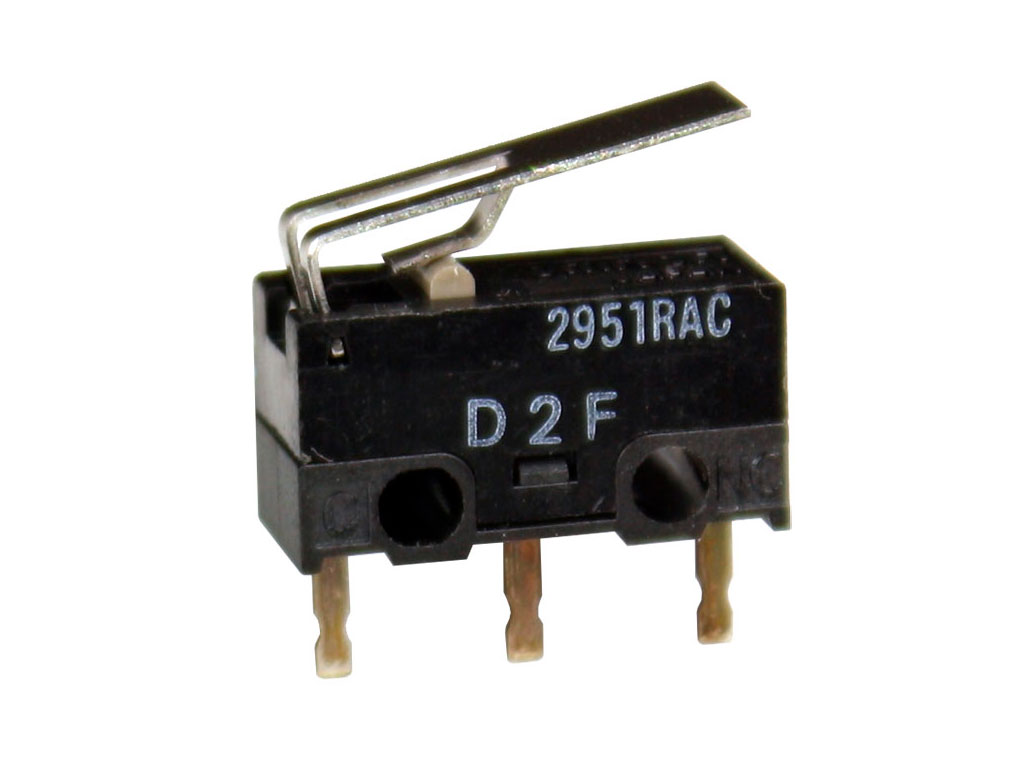
\includegraphics[scale=.3]{it41m01.jpg}
	\caption{Limit Switch.}
\end{figure}

\subsection{RF Transmitter}

This little module is a transmitter among two. It is really simple as it looks. The heart of the module is the SAW resonator which is tuned for 433.xx MHz operation. There is a switching transistor and a few passive components, that’s it.

When a logic HIGH is applied to the DATA input, the oscillator runs producing a constant RF output carrier wave at 433.xx MHz and when the DATA input is taken to logic LOW, the oscillator stops. This technique is known as Amplitude Shift Keying, which we will discuss in detail shortly.

\begin{figure}[h]
	\centering
	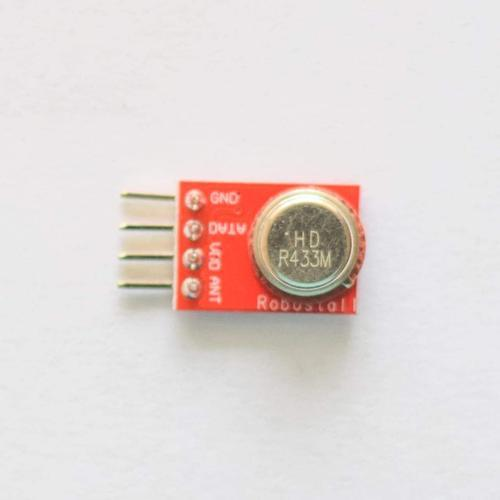
\includegraphics[scale=.3]{512k5yca6zl-_sl1280_-500x500.jpg}
	\caption{RF Transmitter.}
\end{figure}

\subsection{ASK – Amplitude Shift Keying}
For sending the digital data over radio, these modules use a technique called Amplitude Shift Keying or ASK. In Amplitude Shift Keying the amplitude (i.e. the level) of the carrier wave (in our case it’s a 434MHz signal) is changed in response to the incoming data signal.\vspace{.3cm}

This is very similar to the analog technique of amplitude modulation which you might be familiar with if you’re familiar with AM radio. It’s sometimes called binary amplitude shift keying because there are only two levels we are concerned with. You can think of it as an ON/OFF switch.\vspace{.3cm}
\begin{itemize}
	\item For \textbf{Digital 1} – This drives the carrier at full strength.
	\item For\textbf{ Digital 0} – This cuts the carrier off completely.
\end{itemize}
\vspace{.3cm}

This is how the Amplitude modulation looks like:

434MHz RF Transmitter Amplitude Shift Keying ASK Waveform
Amplitude Shift keying has the advantage of being very simple to implement. It is quite simple to design the decoder circuitry. Also ASK needs less bandwidth than other modulation techniques like FSK (Frequency Shift Keying). This is one of the reasons for being inexpensive.\vspace{.3cm}

The disadvantage however is that ASK is susceptible to interference from other radio devices and background noise. But as long as you keep your data transmission to a relatively slow speed it can work reliably in most environments.\vspace{.3cm}

This is how the Amplitude modulation looks like:

\begin{figure}[h]
	\centering
	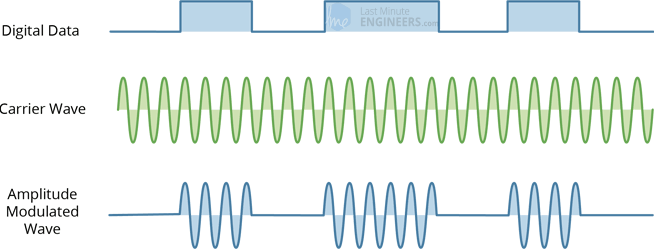
\includegraphics[scale=2.5]{433MHz-RF-Transmitter-Amplitude-Shift-Keying-ASK-Waveform.png}
	\caption{Amplitude Modulation.}
\end{figure}

\subsection{433MHz RF Transmitter Pinout}
Let’s have a look at the pinout of 433MHz RF Transmitter Module.
\begin{figure}[h]
	\centering
	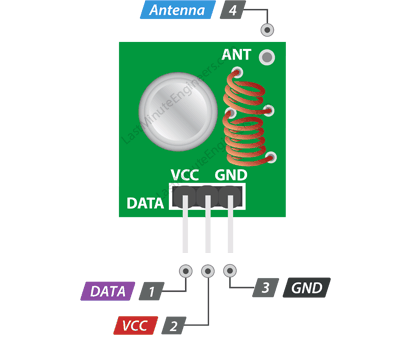
\includegraphics[scale=2.5]{433MHz-RF-Wireless-Transmitter-Pinout.png}
	\caption{RF Transmitter Pin Diagram.}
\end{figure}
\textbf{DATA }pin accepts digital data to be transmitted.

\textbf{VCC }supplies power for the transmitter. This can be any positive DC voltage between 3.5V to 12V. Note that the RF output is proportional to the supply voltage i.e. the higher the Voltage, the greater the range will be.

\textbf{GND} is a ground pin.

\textbf{Antenna} is a pin for external antenna. As discussed earlier, you will want to solder a 17.3 cm piece of solid wire to this pin for the improved range.

\pagebreak
\subsection{RF Transmitter Circuit Diagram}
\begin{figure}[h]
	\centering
	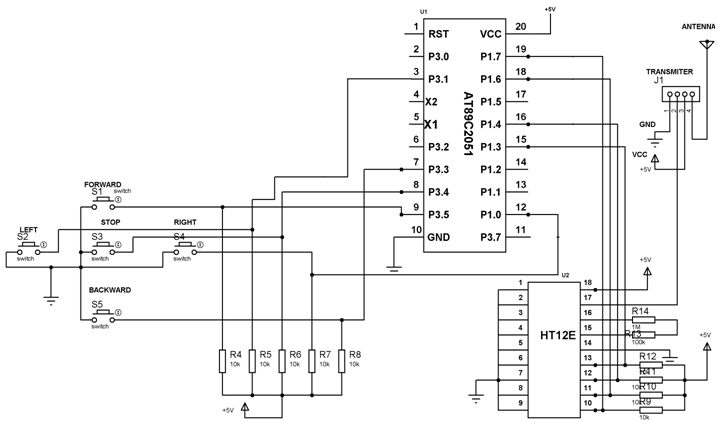
\includegraphics[scale=.6]{RF-Transmitter.png}
	\caption{RF Transmitter Circuit Diagram.}
\end{figure}


\begin{table}[h]
	\begin{center}
		
		%\label{Table 1.1}
		\begin{tabular}{l|l} 
			\textbf{Feature} & \textbf{Value} \\
			\hline
			\textbf{Transmitter frequency range} & 433.92MHz\\
			\textbf{Transmitter supply voltage}	& 3V~6V\\
			\textbf{Transmitter output power} &	4~12Dbm\\
			
			
		\end{tabular}\caption{Features of RF Transmitter.}
	\end{center}
\end{table}

\pagebreak
\subsection{Battery (9 V)}
The nine-volt battery, or 9-volt battery, is a common size of battery that was introduced for the early transistor radios. It has a rectangular prism shape with rounded edges and a polarized snap connector at the top. This type is commonly used in smoke detectors, gas detectors, clocks, walkie-talkies, electric guitars and effects units.\vspace{.3cm}

The nine-volt battery format is commonly available in primary carbon-zinc and alkaline chemistry, in primary lithium iron disulfide, and in rechargeable form in nickel-cadmium, nickel-metal hydride and lithium-ion. Mercury-oxide batteries of this format, once common, have not been manufactured in many years due to their mercury content. Designations for this format include NEDA 1604 and IEC 6F22 (for zinc-carbon) or MN1604 6LR61 (for alkaline). The size, regardless of chemistry, is commonly designated PP3—a designation originally reserved solely for carbon-zinc, or in some countries, E or E-block.\vspace{.3cm}

Most nine-volt alkaline batteries are constructed of six individual 1.5 V LR61 cells enclosed in a wrapper. These cells are slightly smaller than LR8D425 AAAA cells and can be used in their place for some devices, even though they are 3.5 mm shorter. Carbon-zinc types are made with six flat cells in a stack, enclosed in a moisture-resistant wrapper to prevent drying. Primary lithium types are made with three cells in series\vspace{.3cm}

\begin{figure}[h]
	\centering
	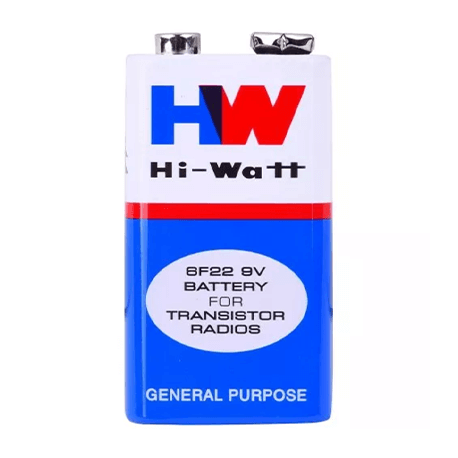
\includegraphics[scale=.3]{9v-Battery-Hi-Watt-long-life-factoryforward-458x458.png}
	\caption{9V Battery.}
\end{figure}
\vspace{.3cm}

The battery has both terminals in a snap connector on one end. The smaller circular (male) terminal is positive, and the larger hexagonal or octagonal (female) terminal is the negative contact. The connectors on the battery are the same as on the load device; the smaller one connects to the larger one and vice versa. The same snap-style connector is used on other battery types in the Power Pack (PP) series. Battery polarization is normally obvious, since mechanical connection is usually only possible in one configuration.

\subsection{Diode}
One of the first semiconductor based engineering components, diodes are an indispensible necessity for any current modern gadget or circuit. They are the basic logic block – the most fundamental unit.\vspace{.3cm}

These two terminal-ed nonlinear passive elements ideally conduct only one way and hence protect the circuit as well as the source from any damage. Diodes are widely used in rectifier circuits, limiters, communication circuits, multiplier circuits and signal clippers as well as clamper circuits. This Insight will give an in depth view of a diode’s physicality.

The core of the diode is enclosed in an epoxy that protects the semiconductor from ambient adversities. This epoxy molding is black colored, marked with the diode number on the center and a silver colored band at one end – the band labeling that end to be the diode’s cathode. Connected to the epoxy at both the ends are two electroplated leads. These leads are able to withstand high temperatures and provide good soldering properties.
\begin{figure}[h]
	\centering
	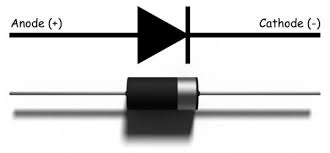
\includegraphics[scale=.3]{download.jpg}
	\caption{Diode.}
	
	
\end{figure}
\subsection{Capacitor}
Capacitor is a passive component used to store charge. The charge (q) stored in a capacitor is the product of its capacitance (C) value and the voltage (V) applied to it. Capacitors offer infinite reactance to zero frequency so they are used for blocking DC components or bypassing the AC signals. The capacitor undergoes through a recursive cycle of charging and discharging in AC circuits where the voltage and current across it depends on the RC time constant. For this reason, capacitors are used for smoothing power supply variations. Other uses include, coupling the various stages of audio system, tuning in radio circuits etc. These are used to store energy like in a camera flash.

\begin{figure}[h]
	\centering
	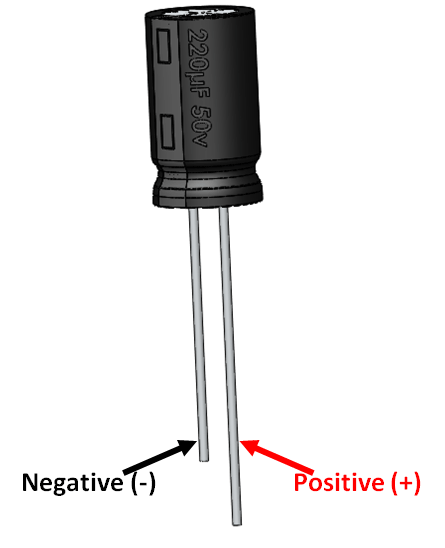
\includegraphics[scale=.5]{electrolytic-capacitor-pinout.png}
	\caption{Capacitor.}
\end{figure}


Capacitors may be non-polarized/polarized and fixed/variable. Electrolytic capacitors are polarized while ceramic and paper capacitors are examples of non polarized capacitors. Since capacitors store charge, they must be carefully discharged before troubleshooting the circuits. The maximum voltage rating of the capacitors used must always be greater than the supply voltage. Click to learn more about working of a capacitor along with its internal structure.

\subsection{HT12E}
HT12E is an encoder IC for RF and IR modules mostly. It is a 12-bit decoder that uses 8-bits for address and 4 for data. RF and IR modules can interface with microcontrollers directly which requires a little bit complex programming. In addition, This encoder IC is easy to implement and simple to use. It comes in 18 and 20 pins. Both packages have only 18 functional pins. Furthermore, This encoder will use the logic states as data and address inputs. HT12E doesn’t work alone. It’s only an encoder and one side of communicator. On the contrary,  the second part of the communicator uses an HT12D decoder. In short, HT12D is the most suitable decoder for HT12E because both are 12-bits and have the same number of address and data pins.
\begin{figure}[h]
	\centering
	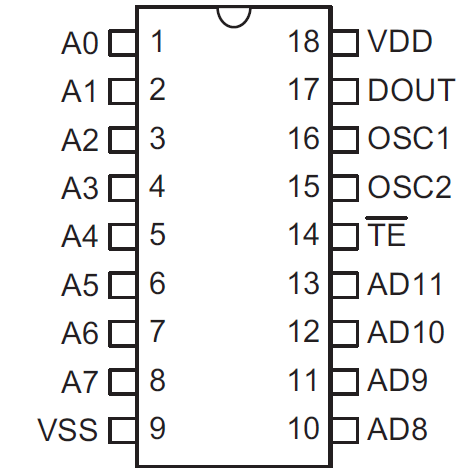
\includegraphics[scale=.5]{HT12E-Encoder-Pinout-diagram-Configuration.png}
	\caption{HT12E Pinout Diagram.}
\end{figure}
\pagebreak
\section{Bike Section}

The Vehicle Unit is a part of the actual two-wheeler. It is wirelessly connected to the Helmet Unit and it can be placed anywhere on the motor-bike preferably at a position which is less prone to the damage.\vspace{.3cm}



The Vehicle Unit is also powered with the battery with the recharging capacity. The unit comprises a section for keeping the battery and a USB port so that it will provide the recharging sobriety to the unit as shown. It also includes a battery level indicator which actually indicates the amount of charge which is left in the unit to operate. The microcontroller is connected to the battery for the supply of the power. This microcontroller receives the signals from the microcontroller in the Helmet Unit and then it further processes the received information. The microcontroller and the ignition key switch are connected to each other via a relay module (1 channel 5V relay module) which actually controls the ignition of the vehicle which is based on the values received from the controller.

\begin{figure}[h]
	\centering
	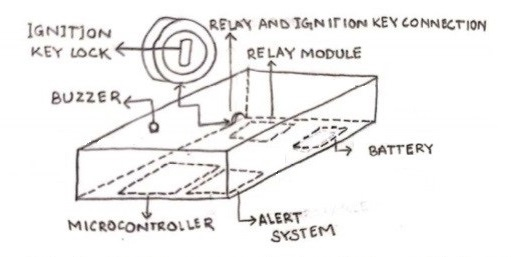
\includegraphics[scale=1.3]{Vehicle unit.jpg}
	\caption{Proposed Bike Section.}
\end{figure}\vspace{.3cm}

\textbf{The elements in bike section are explained as follows:}

\subsection{RF Receiver}
This one is a receiver module. Though it looks complex, it is as simple as the transmitter module. It consists of a RF tuned circuit and a couple of OP Amps to amplify the received carrier wave from the transmitter. The amplified signal is further fed to a PLL (Phase Lock Loop) which enables the decoder to “lock” onto a stream of digital bits which gives better decoded output and noise immunity

\begin{figure}[h]
	\centering
	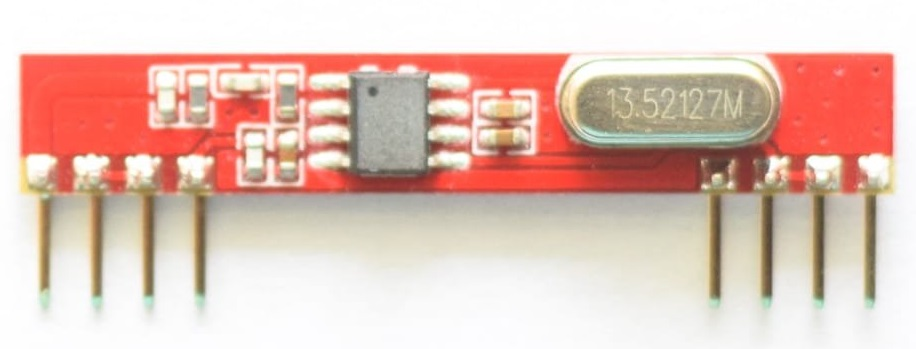
\includegraphics[scale=.4]{51JDasXMQAL._SL1176_.jpg}
	\caption{RF Receiver.}
\end{figure}

\begin{table}[h]
	\begin{center}
		
		%\label{Table 1.1}
		\begin{tabular}{l|l} 
			\textbf{Feature} & \textbf{Value} \\
			\hline
			\textbf{Receiver frequency} & 433MHz\\
			\textbf{Receiver typical frequency }	& 105Dbm\\
			\textbf{Receiver supply current} & 3.5mA\\
			
			
		\end{tabular}
		\caption{Features of RF Reciever.}
	\end{center}
\end{table}
\subsection{RF Reciever Circuit Diagram}
\begin{figure}[h]
	\centering
	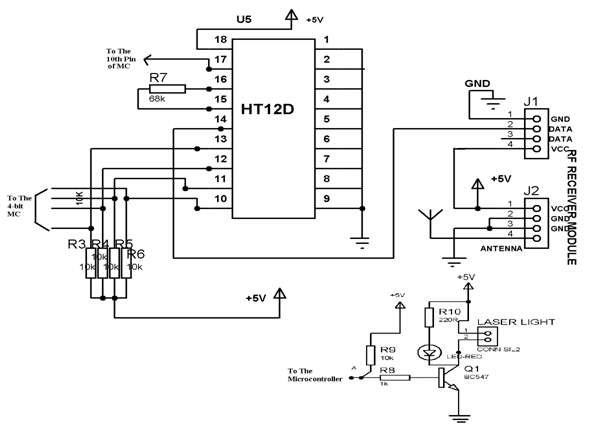
\includegraphics[scale=.65]{RF-Receiver.png}
	\caption{RF Receiver Circuit Diagram.}
\end{figure}


\subsection{Reed Switch}
The reed switch is an electrical switch operated by an applied magnetic field. It was invented at Bell Telephone Laboratories in 1936 by W. B. Ellwood.\vspace{.3cm}

\textbf{Reed Switch Principle}\vspace{.3cm}

It consists of a pair of contacts on ferrous metal reeds in a hermetically sealed glass envelope. The contacts may be normally open, closing when a magnetic field is present, or normally closed and opening when a magnetic field is applied.\vspace{.3cm}

The switch may be actuated by a coil, making a reed relay, or by bringing a magnet near to the switch. Once the magnet is pulled away from the switch, the reed switch will go back to its original position.\vspace{.3cm}

\begin{figure}[h]
	\centering
	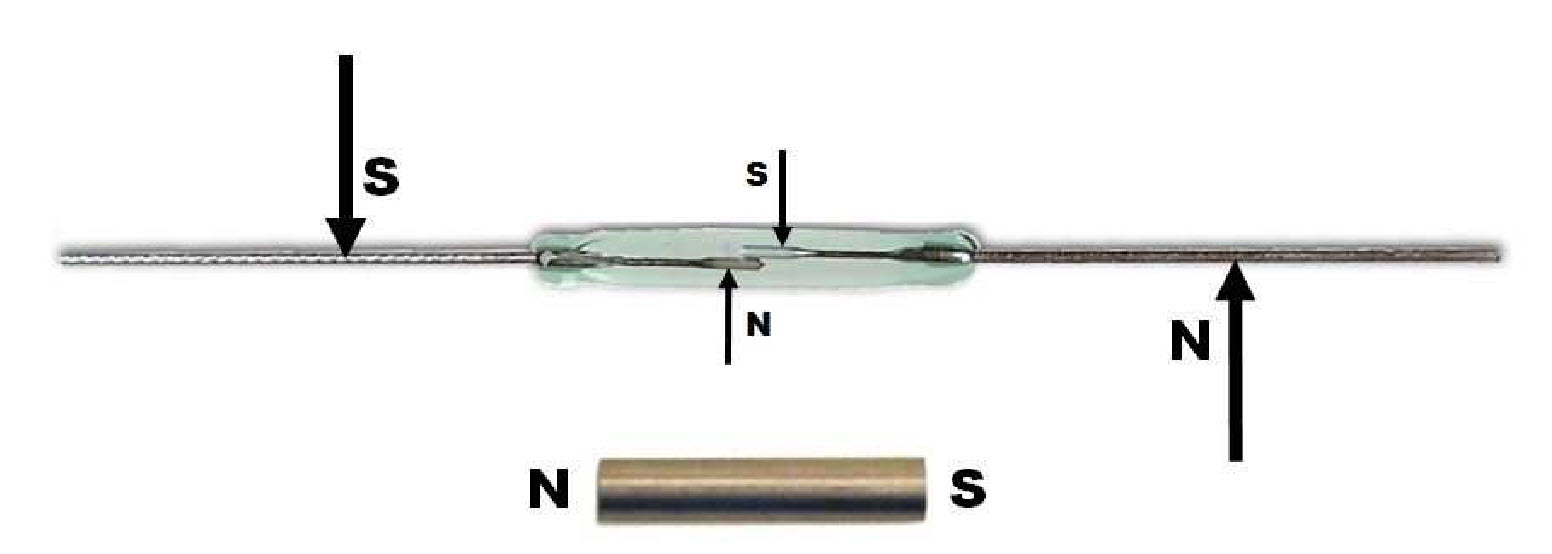
\includegraphics[scale=.35]{Figure-2-Reed-switch.jpg}
	\caption{Reed Switch.}
\end{figure}
\subsection{Reed switches Operation}
The simplest magnetic-field sensor is a reed switch. It contains two ferromagnetic nickel and iron reed elements in an evacuated, hermetically sealed glass tube to minimize contact arcing.\vspace{.3cm}

When an axially aligned magnet approaches the switch, its magnetic force closes the reeds. The magnet typically generates at least a 50 Gauss force to overcome the return force or spring of the reed elements.\vspace{.3cm}

Reed switches are inexpensive, require no standby power, and can function with both ac and dc electrical loads. However, they are relatively slow, so they may not respond fast enough for some high-speed applications.\vspace{.3cm}



Since the switches are mechanical devices with moving parts, they have a finite number of operating cycles before they eventually fail. Switching high-current loads can further reduce life expectancy.\vspace{.3cm}

Also, low-cost reed switches occasionally deliver unwanted, multiple switching points as the twin lobes of certain magnets pass by.\vspace{.3cm}


\begin{figure}[h]
	\centering
	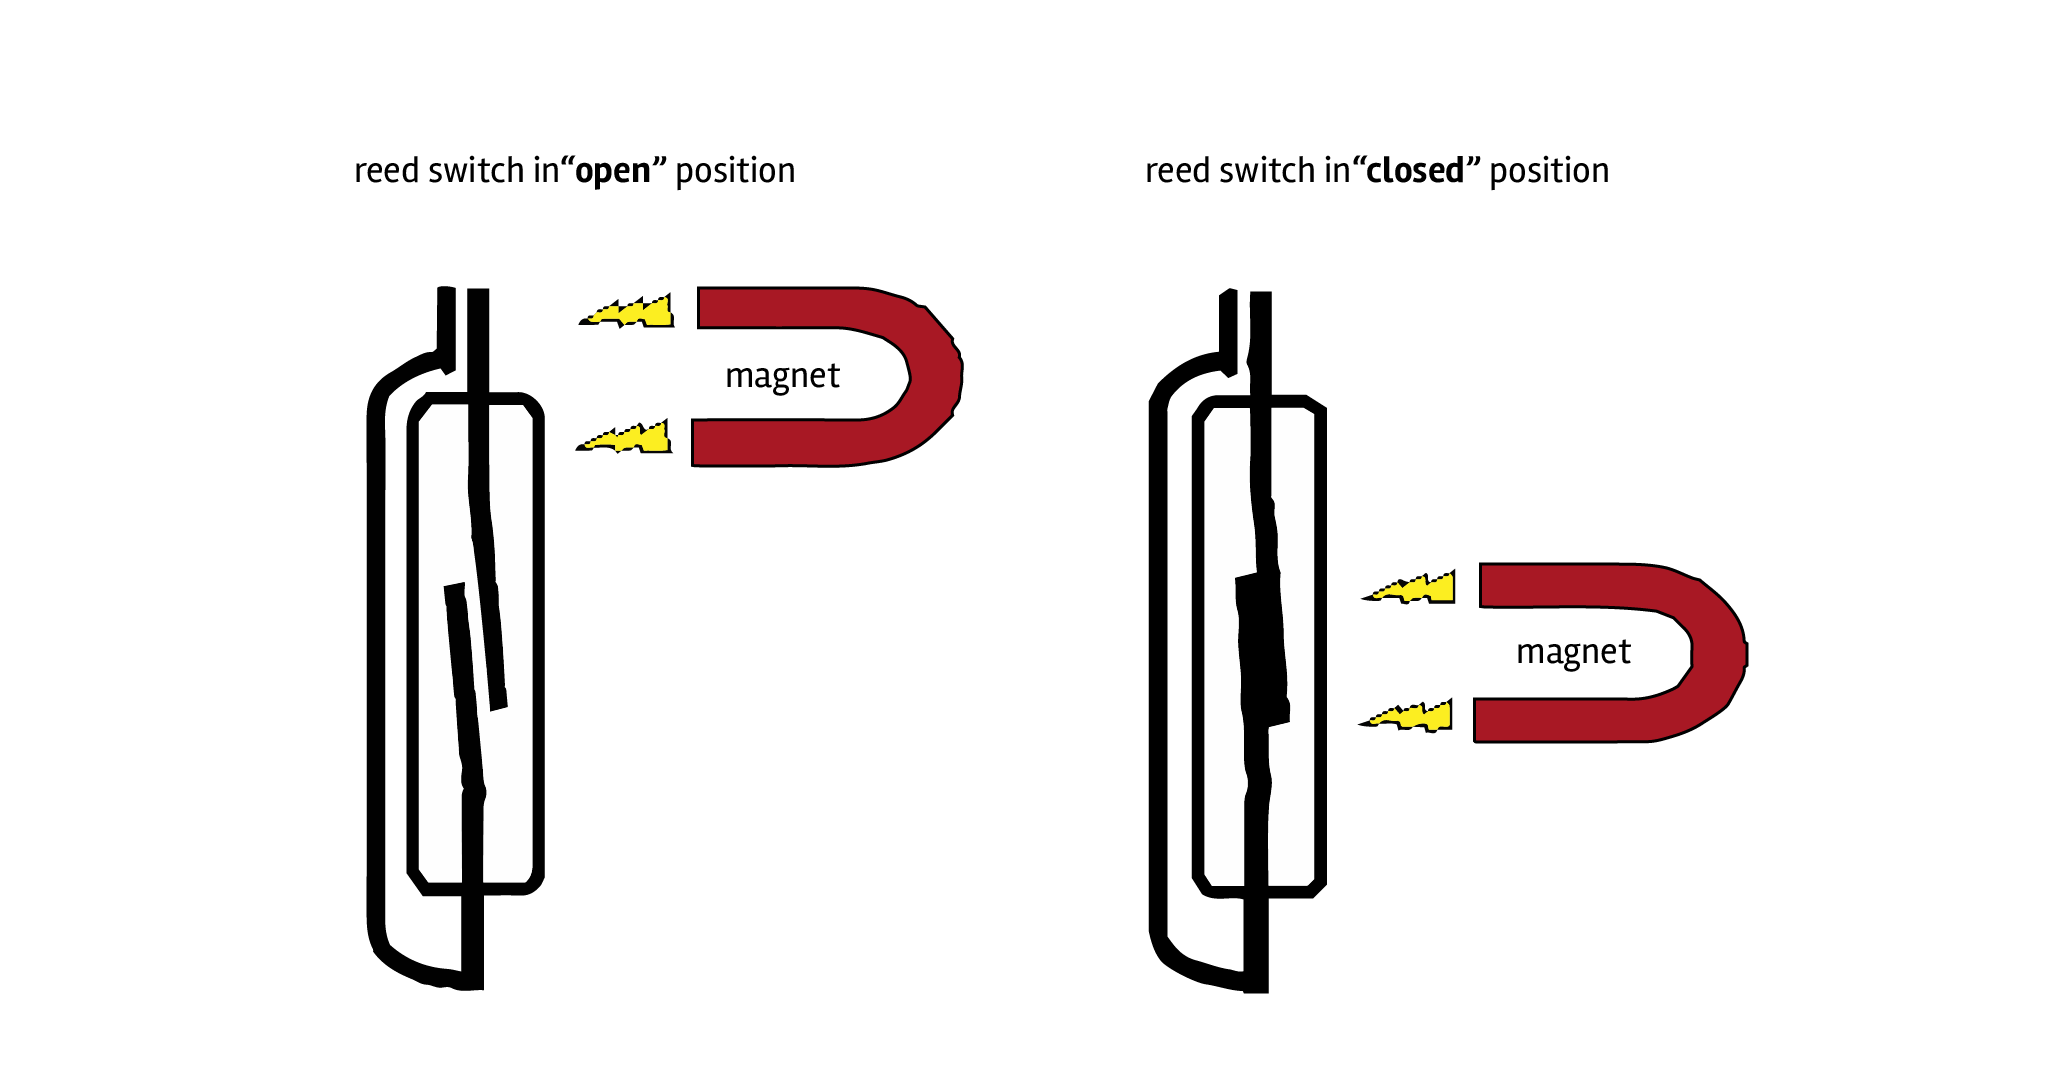
\includegraphics[scale=.15]{Reed-switches_2.png}
	\caption{Reed Switch Working.}
\end{figure}

\subsection{Sim 800L GSM Module}
GSM/GPRS module is used to establish communication between a computer and
a GSM-GPRS system. Global System for Mobile communication (GSM) is an
architecture used for mobile communication in most of the countries. Global Packet
Radio Service (GPRS) is an extension of GSM that enables higher data transmission
rate.GSM/GPRS module consists of a GSM/GPRS modem assembled together
with power supply circuit and communication interfaces (like RS-232, USB, etc) for
computer. The MODEM is the soul of such modules.\\
Sim800L Module is low cost, low form factor GSM module based on Simcoms SIM800L chipset. Sim800L module supports quad-band GSM and GPRS network.
This breakout board is perfect for application where size and cost is a constraint. Sim800l gsm module also supports quad band which means that it can work anywhere in the world. This low cost module is perfect for launching your next IoT project. Using this module you can almost make your own cellphone. 

\subsection*{Using this module you can:-}
\begin{itemize}
	\item Send Text Messages (SMS)
	\item Make or receive Phone calls
	\item Connect to Internet via GPRS
	\item TCP/IP
\end{itemize}

The main drawback of this module is works on 3.7 to 4.2 volts so you cannot power it directly through Arduino or Raspberry Pi. Moreover the sim800L GSM and GPRS module requires upto 2 ampere current so accordingly design your power supply. You can use a 3.7 volt lipo battery to directly power the GSM module.\vspace{.3cm}

You can communicate with SIM800l module via UART port, supports command including 3GPP TS 27.007, 27.005 and SIM COM enhanced AT Commands.

\subsection*{Features of SIM800L GSM Module:-}
\begin{itemize}
	\item Quad-band 850/900/1800/1900MHz - connect onto any global GSM network with any 2G SIM (in the USA, T-Mobile is suggested).
	\item Make and receive voice calls using a headset or an external 8 Ohm speaker and electret microphone.
	\item PWM/Buzzer vibration motor control
	\item AT command interface with "auto baud" detection
	\item Send and receive SMS messages.
	\item Send and receive GPRS data (TCP/IP, HTTP, etc.).
	\item Scan and receive FM radio broadcasts.
	\item Lead out buzzer and vibration motor control port.
	\item AT command interface with "auto baud" detection.
	\item Onboard IPEX socket that can be connected to external antenna.
	\item Breakouts for external 8W speaker and electret mic if you don't want to use a headphone
	\item Level shifting circuitry so you can run it with 2.8V to 5V logic.
	\item Vibrational motor (buzzer) driver so you can have noiseless notifications
	\item uFL or SMA connections for external antenna
	\item Indicator LEDs for power and network connectivity
	\item Standard SIM slides into the back
\end{itemize}
\pagebreak	
\begin{figure}[h]
	\centering
	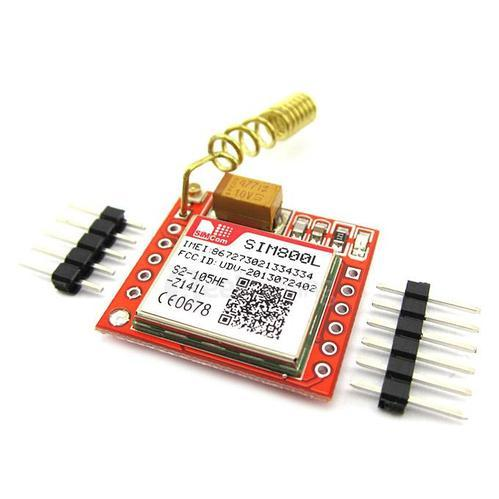
\includegraphics[scale=.6]{gsm-sim800l-module-500x500.jpg}
	\caption{SIM 800L GSM Module.}
\end{figure}
\subsection{Relay Switch}
Relay is an electromagnetic device which is used to isolate two circuits electrically
and connect them magnetically. They are very useful devices and allow one circuit
to switch another one while they are completely separate. They are often used to
interface an electronic circuit (working at a low voltage) to an electrical circuit
which works at very high voltage. For example, a relay can make a 5V DC battery
circuit to switch a 230V AC mains circuit. Thus a small sensor circuit can drive, say,
a fan or an electric bulb.\vspace{.3cm}

A relay switch can be divided into two parts: input and output. The input section
has a coil which generates magnetic field when a small voltage from an electronic
circuit is applied to it. This voltage is called the operating voltage. Commonly used
relays are available in different configuration of operating voltages like 6V, 9V,
12V, 24V etc. The output section consists of contactors which connect or
disconnect mechanically. In a basic relay there are three contactors: normally
open (NO), normally closed (NC) and common (COM). At no input state, the COM
is connected to NC. When the operating voltage is applied the relay coil gets
energized and the COM changes contact to NO. Different relay configurations are
available like SPST, SPDT, DPDT etc, which have different number of changeover
contacts. By using proper combination of contactors, the electrical circuit can be
switched on and off. Get inner details about structure of a relay switch.
\begin{figure}[h]
	\centering
	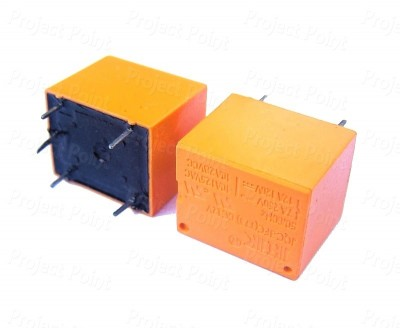
\includegraphics[scale=.6]{RELAY 12V.jpeg}
	\caption{Relay Switch.}
\end{figure}


\pagebreak\subsection{12 V DC Motor}
A DC motor is any motor within a class of electrical machines whereby direct current electrical power is converted into mechanical power. Most often, this type of motor relies on forces that magnetic fields produce. Regardless of the type, DC motors have some kind of internal mechanism, which is electronic or electromechanical. In both cases, the direction of current flow in part of the motor is changed periodically.\vspace{.3cm}

The speed of a DC motor is controlled using a variable supply voltage or by changing the strength of the current within its field windrings. While smaller DC motors are commonly used in the making of appliances, tools, toys, and automobile mechanisms, such as electric car seats, larger DC motors are used in hoists, elevators, and electric vehicles.\vspace{.3 cm}

A 12v DC motor is small and inexpensive, yet powerful enough to be used for many applications. Because choosing the right DC motor for a specific application can be challenging, it is important to work with the right company. A prime example is METMotors, which has been creating high-quality permanent magnet DC motors for more than 45 years.\vspace{.3cm}
\begin{figure}[h]
	\centering
	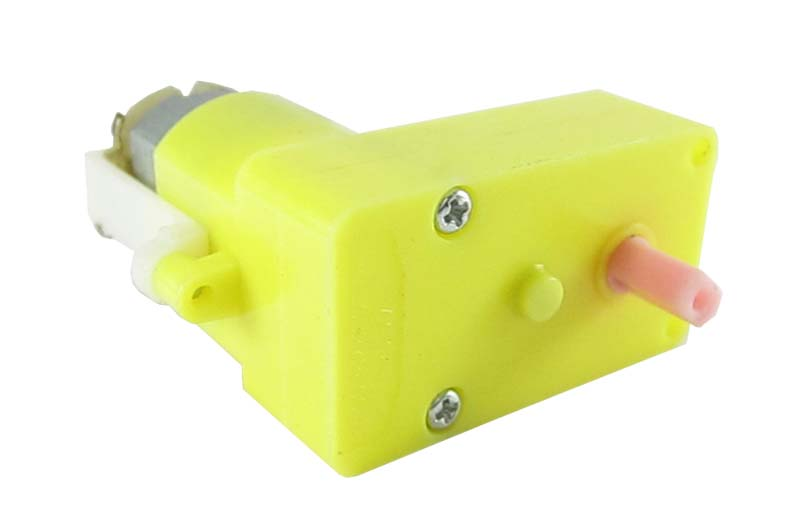
\includegraphics[scale=.4]{1B.jpg}
	\caption{12V DC Motor.}
\end{figure}


\subsection{LED}
Light emitting diodes (LEDs) are semiconductor light sources. The light emitted
from LEDs varies from visible to infrared and ultraviolet regions. They operate on low
voltage and power. LEDs are one of the most common electronic components and are
mostly used as indicators in circuits. They are also used for luminance and
optoelectronic applications.\vspace{.3cm}
\begin{figure}[h]
	\centering
	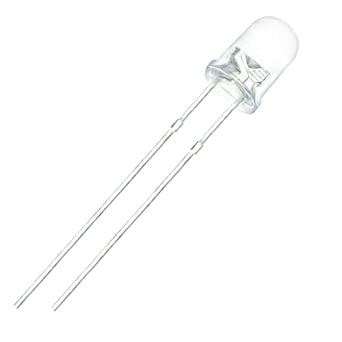
\includegraphics[scale=.4]{417ofv1fVpL._SX342_.jpg}
	\caption{LED.}
\end{figure}
Based on semiconductor diode, LEDs emit photons when electrons recombine with
holes on forward biasing. The two terminals of LEDs are anode (+) and cathode (-) and
can be identified by their size. The longer leg is the positive terminal or anode and
shorter one is negative terminal.\vspace{.3cm}


The forward voltage of LED (1.7V-2.2V) is lower than the voltage supplied (5V) to drive
it in a circuit. Using an LED as such would burn it because a high current would destroy
its p-n gate. Therefore a current limiting resistor is used in series with LED. Without this
resistor, either low input voltage (equal to forward voltage) or PWM (pulse width
modulation) is used to drive the LED. Get details about internal structure of a LED.\vspace{.3cm}
\begin{figure}[h]
	\centering
	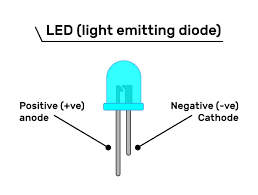
\includegraphics[scale=.9]{download.png}
	\caption{LED Pin Diagram.}
\end{figure}





\subsection{LCD Display}
LCD (Liquid Crystal Display) screen is an electronic display module and find a wide
range of applications. A 16x2 LCD display is very basic module and is very commonly
used in various devices and circuits. These modules are preferred over seven
segments and other multi segment LEDs. The reasons being: LCDs are economical;
easily programmable; have no limitation of displaying special \&amp; even custom
characters (unlike in seven segments),animations and so on.
A 16x2 LCD means it can display 16 characters per line and there are 2 such lines. In
this LCD each character is displayed in 5x7 pixel matrix. This LCD has two registers,
namely, Command and Data.
The command register stores the command instructions given to the LCD. A command
is an instruction given to LCD to do a predefined task like initializing it, clearing its
screen, setting the cursor position, controlling display etc. The data register stores the

data to be displayed on the LCD. The data is the ASCII value of the character to be
displayed on the LCD. Click to learn more about internal structure of a LCD.

\begin{figure}[h]
	\centering
	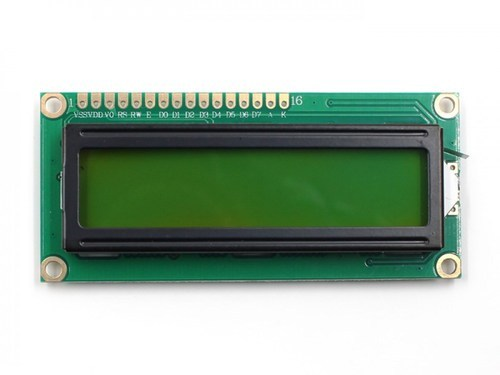
\includegraphics[scale=.4]{16x2-lcd-display-green-500x500.jpg}
	\caption{LCD Display.}
\end{figure}
\pagebreak
\textbf{Pin Description}

\begin{table}[h]
	\begin{center}
		
		%\label{Table 1.1}
		\begin{tabular}{l|l|l} 
			\textbf{Pin No.} & \textbf{Function} & \textbf{Name} \\
			\hline
			\textbf{1} & Ground (0V) & Ground\\
			\textbf{2} & Supply voltage; 5V (4.7V-5.3V) & Vcc\\
			\textbf{3} & Contrast adjustment; through avariable resistor &Vee/Contrast \\
			\textbf{4} & Selects command register when low; and data register when high &Register Select \\
			\textbf{5} &Low to write to the register5; High to read from the register  &Read/Write \\
			\textbf{6} & Sends data to data pins when a high to low pulse is given & Enable\\
			\textbf{7} & 8-bit data pins &DB0 \\
			\textbf{8} & 8-bit data pins &DB1 \\
			\textbf{9} & 8-bit data pins &DB2 \\
			\textbf{10} & 8-bit data pins &DB3 \\
			\textbf{11} & 8-bit data pins &DB4 \\
			\textbf{12} & 8-bit data pins &DB5 \\
			\textbf{13} & 8-bit data pins &DB6 \\
			\textbf{14} & 8-bit data pins &DB7 \\
			\textbf{15} & Backlight Vcc (5V) &Backlight (+) \\
			\textbf{16} & Backlight Ground (0V) &Backlight (-) \\
			
		\end{tabular}
		\caption{Pin Description.}
	\end{center}
\end{table}
\begin{figure}[h]
	\centering
	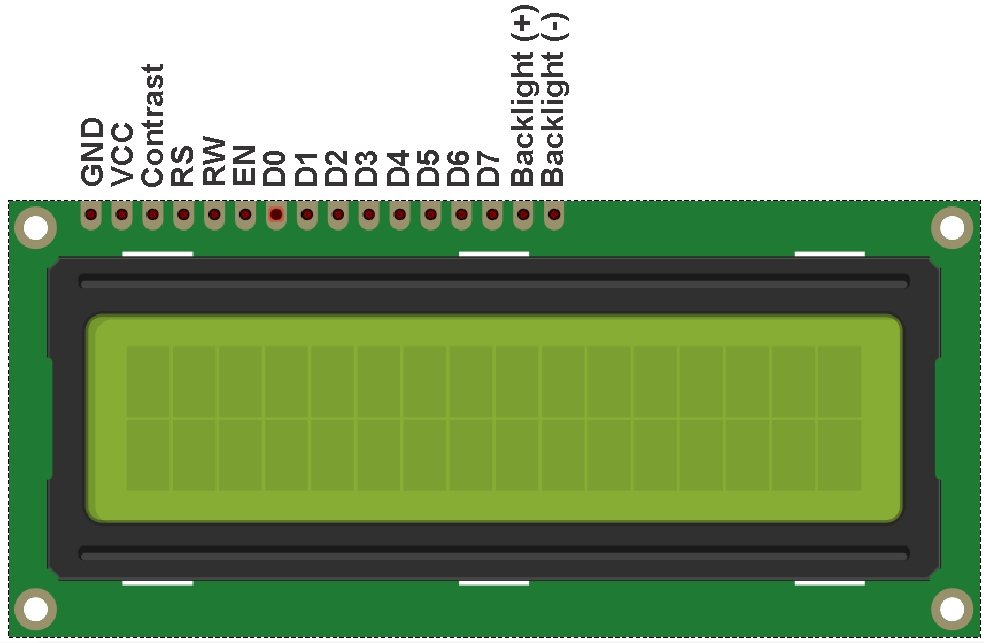
\includegraphics[scale=.4]{16x2-LCD-Display-Pin-Description.jpg}
	\caption{LCD Display Pin Diagram.}
\end{figure}



\pagebreak
\subsection{Arduino UNO}
Arduino is a prototype platform (open-source) based on an easy-to-use hardware and software. It consists of a circuit board, which can be programed (referred to as a microcontroller) and a ready-made software called Arduino IDE (Integrated Development Environment), which is used to write and upload the computer code to the physical board.\vspace{.3cm}

\textbf{The key features are: }
\begin{itemize}
	\item Arduino boards are able to read analog or digital input signals from different sensors and turn it into an output such as activating a motor, turning LED on/off, connect to the cloud and many other actions.
	
	\item You can control your board functions by sending a set of instructions to the microcontroller on the board via Arduino IDE (referred to as uploading software).
	
	\item Unlike most previous programmable circuit boards, Arduino does not need an extra piece of hardware (called a programmer) in order to load a new code onto the board. You can simply use a USB cable.
	
	\item Additionally, the Arduino IDE uses a simplified version of C++, making it easier to learn to program.
	
	\item Finally, Arduino provides a standard form factor that breaks the functions of the micro-controller into a more accessible package.
\end{itemize}
\begin{figure}[h]
	\centering
	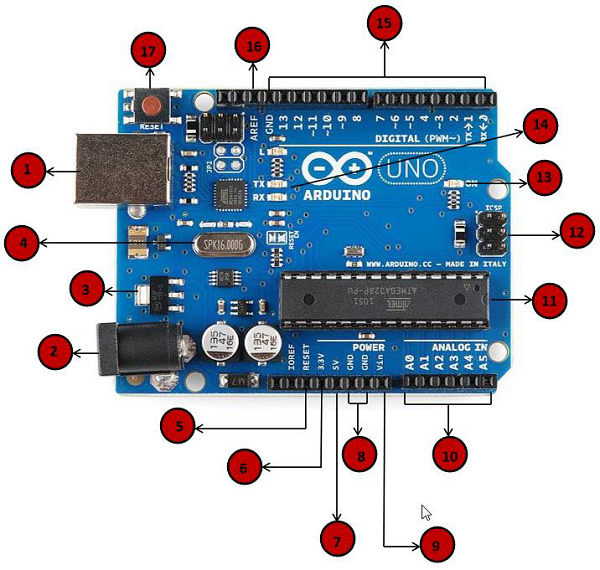
\includegraphics[scale=.7]{board_description.png}
	\caption{Arduino UNO.}
\end{figure}

\textbf{1: Power USB}\vspace{.3cm}

Arduino board can be powered by using the USB cable from your computer. All you need to do is connect the USB cable to the USB connection (1).\vspace{.3cm}

\textbf{2: Power (Barrel Jack)}\vspace{.3cm}

Arduino boards can be powered directly from the AC mains power supply by connecting it to the Barrel Jack (2).\vspace{.3cm}

\textbf{3: Voltage Regulator}\vspace{.3cm}

The function of the voltage regulator is to control the voltage given to the Arduino board and stabilize the DC voltages used by the processor and other elements.\vspace{.3cm}

\textbf{4: Crystal Oscillator}\vspace{.3cm}

The crystal oscillator helps Arduino in dealing with time issues. How does Arduino calculate time? The answer is, by using the crystal oscillator. The number printed on top of the Arduino crystal is 16.000H9H. It tells us that the frequency is 16,000,000 Hertz or 16 MHz.\vspace{.3cm}

\textbf{5,17: Arduino Reset}\vspace{.3cm}

You can reset your Arduino board, i.e., start your program from the beginning. You can reset the UNO board in two ways. First, by using the reset button (17) on the board. Second, you can connect an external reset button to the Arduino pin labelled RESET (5).\vspace{.3cm}

\textbf{6,7,8,9: Pins (3.3, 5, GND, Vin)}\vspace{.3cm}

\begin{itemize}
	\item 3.3V (6) :- Supply 3.3 output volt
	
	\item 5V (7) :- Supply 5 output volt
	
	\item Most of the components used with Arduino board works fine with 3.3 volt and 5 volt.
	
	\item GND (8)(Ground) :- There are several GND pins on the Arduino, any of which can be used to ground your circuit.
	
	\item Vin (9) :- This pin also can be used to power the Arduino board from an external power source, like AC mains power supply.
\end{itemize}\vspace{.3cm}

\textbf{10: Analog pins}\vspace{.3cm}

The Arduino UNO board has six analog input pins A0 through A5. These pins can read the signal from an analog sensor like the humidity sensor or temperature sensor and convert it into a digital value that can be read by the microprocessor.\vspace{.3cm}

\textbf{11: Main microcontroller}\vspace{.3cm}

Each Arduino board has its own microcontroller (11). You can assume it as the brain of your board. The main IC (integrated circuit) on the Arduino is slightly different from board to board. The microcontrollers are usually of the ATMEL Company. You must know what IC your board has before loading up a new program from the Arduino IDE. This information is available on the top of the IC. For more details about the IC construction and functions, you can refer to the data sheet.\vspace{.3cm}

\textbf{12: ICSP pin}\vspace{.3cm}

Mostly, ICSP (12) is an AVR, a tiny programming header for the Arduino consisting of MOSI, MISO, SCK, RESET, VCC, and GND. It is often referred to as an SPI (Serial Peripheral Interface), which could be considered as an "expansion" of the output. Actually, you are slaving the output device to the master of the SPI bus.\vspace{.3cm}

\textbf{13:Power LED indicator}\vspace{.3cm}

This LED should light up when you plug your Arduino into a power source to indicate that your board is powered up correctly. If this light does not turn on, then there is something wrong with the connection.\vspace{.3cm}

\textbf{14: TX and RX LEDs}\vspace{.3cm}

On your board, you will find two labels: TX (transmit) and RX (receive). They appear in two places on the Arduino UNO board. First, at the digital pins 0 and 1, to indicate the pins responsible for serial communication. Second, the TX and RX led (13). The TX led flashes with different speed while sending the serial data. The speed of flashing depends on the baud rate used by the board. RX flashes during the receiving process.\vspace{.3cm}

\textbf{15: Digital I/O}\vspace{.3cm}

The Arduino UNO board has 14 digital I/O pins (15) (of which 6 provide PWM (Pulse Width Modulation) output. These pins can be configured to work as input digital pins to read logic values (0 or 1) or as digital output pins to drive different modules like LEDs, relays, etc. The pins labeled “~” can be used to generate PWM.\vspace{.3cm}

\textbf{16: AREF}\vspace{.3cm}

AREF stands for Analog Reference. It is sometimes, used to set an external reference voltage (between 0 and 5 Volts) as the upper limit for the analog input pins.


\subsection{ATmega 328P IC}
\begin{itemize}
	\item ATmega328 is an 8-bit, 28-Pin AVR Microcontroller, manufactured by Microchip, follows RISC Architecture and has a flash-type program memory of 32KB.
	\item Atmega328 is the microcontroller, used in basic Arduino boards i.e Arduino UNO, Arduino Pro Mini and Arduino Nano.
	\item It has an EEPROM memory of 1KB and its SRAM memory is 2KB.
	\item It has 8 Pins for ADC operations, which all combine to form PortA ( PA0 - PA7 ).
	\item It also has 3 built-in Timers, two of them are 8 Bit timers while the third one is 16-Bit Timer.
	\item You must have heard of Arduino UNO, UNO is based on atmega328 Microcontroller. It's UNO's heart. :)
	\item It operates ranging from 3.3V to 5.5V but normally we use 5V as a standard.
	\item Its excellent features include cost-efficiency, low power dissipation, programming lock for security purposes, real timer counter with separate oscillator.
	\item It's normally used in Embedded Systems applications. You should have a look at these Real Life Examples of Embedded Systems, we can design all of them using this Microcontroller.
\end{itemize}

\begin{figure}[h]
	\centering
	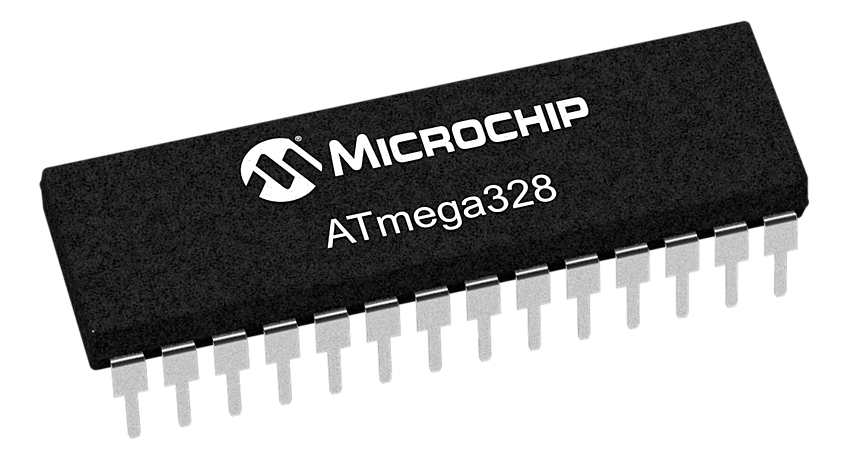
\includegraphics[scale=.5]{High-quality-electronic-components-atmega328-for-distributors.png}
	\caption{ATmega 328P IC.}
\end{figure}

\textbf{ATmega328 Pins Description}
\begin{itemize}
	\item Functions associated with the pins must be known in order to use the device appropriately.
	\item ATmega-328 pins are divided into different ports which are given in detail below.
	\item VCC is a digital voltage supply.
	\item AVCC is a supply voltage pin for analog to digital converter.
	\item GND denotes Ground and it has a 0V.
	\item Port A consists of the pins from PA0 to PA7. These pins serve as an analog input to analog to digital converters. If analog to digital converter is not used, port A acts as an eight (8) bit bidirectional input/output port.
	\item Port B consists of the pins from PB0 to PB7. This port is an 8 bit bidirectional port having an internal pull-up resistor.
	\item Port C consists of the pins from PC0 to PC7. The output buffers of port C has symmetrical drive characteristics with source capability as well high sink.
	\item Port D consists of the pins from PD0 to PD7. It is also an 8 bit input/output port having an internal pull-up resistor.
	\item All of the AVR ports are shown in the figure given below.
\end{itemize}
\begin{figure}[h]
	\centering
	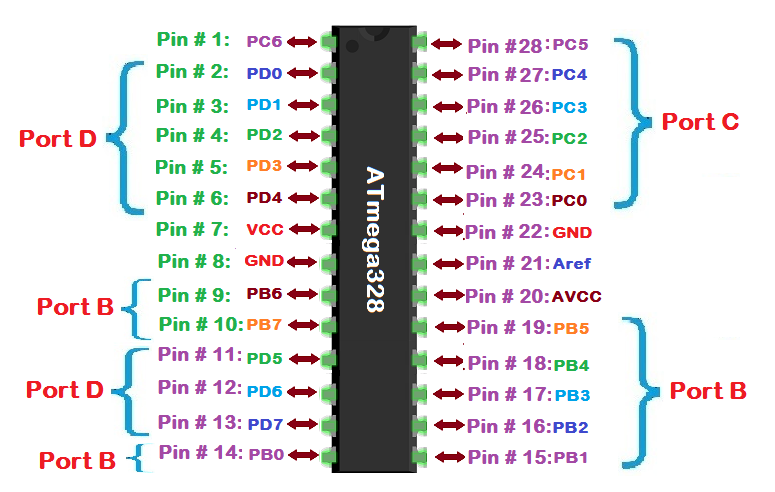
\includegraphics[scale=.42]{ATmega328-Ports.png}
	\caption{ATmega 328 Ports.}
\end{figure}
\textbf{The following table shows the complete features of ATmega328:}

\begin{table}[h]
	\begin{center}
		
		%\label{Table 1.1}
		\begin{tabular}{l|l} 
			\textbf{Feature} & \textbf{Description} \\
			\hline
			\textbf{1} & Ground (0V) \\
			No. of Pins	& 28]\\
			CPU	& RISC 8-Bit AVR\\
			Operating Voltage	& 1.8 to 5.5 V\\
			Program Memory	& 32KB\\
			Program Memory Type	& Flash\\
			SRAM	& 2048 Bytes\\
			EEPROM	& 1024 Bytes\\
			ADC	& 10-Bit\\
			Number of ADC Channels	& 8\\
			PWM Pins	& 6\\
			Comparator	& 1\\
			Packages (4)	& 8-pin PDIP32-lead TQFP28-pad QFN/MLF32-pad QFN/MLF\\
			Oscillator	& up to 20 MHz\\
			Timer (3)	& 8-Bit x 2 \& 16-Bit x 1\\
			Enhanced Power-on Reset	& Yes\\
			Power Up Timer	& Yes\\
			I/O Pins	& 23\\
			Manufacturer	& Microchip\\
			SPI	& Yes\\
			I2C	& Yes\\
			Watchdog Timer	& Yes\\
			Brownout detect (BOD)	& Yes\\
			Reset	& Yes\\
			USI (Universal Serial Interface)	& Yes\\
			Minimum Operating Temperature	& -40 C to +85 C\\
			
		\end{tabular}
		\caption{ATmega328 Features.}
	\end{center}
\end{table}


\pagebreak
\subsection{Buzzer}
A buzzer is a small yet efficient component to add sound features to our project/system. It is very small and compact 2-pin structure hence can be easily used on breadboard, Perf Board and even on PCBs which makes this a widely used component in most electronic applications.\vspace{.3cm}

There are two types are buzzers that are commonly available. The one shown here is a simple buzzer which when powered will make a Continuous Beeeeeeppp.... sound, the other type is called a readymade buzzer which will look bulkier than this and will produce a Beep. Beep. Beep. Sound due to the internal oscillating circuit present inside it. But, the one shown here is most widely used because it can be customised with help of other circuits to fit easily in our application.\vspace{.3cm}

This buzzer can be used by simply powering it using a DC power supply ranging from 4V to 9V. A simple 9V battery can also be used, but it is recommended to use a regulated +5V or +6V DC supply. The buzzer is normally associated with a switching circuit to turn ON or turn OFF the buzzer at required time and require interval.\vspace{.3cm}
\begin{figure}[h]
	\centering
	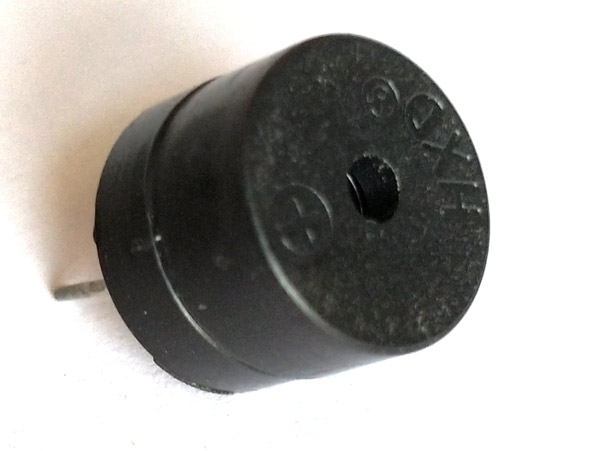
\includegraphics[scale=.5]{Buzzer.jpg}
	\caption{Buzzer.}
\end{figure}\vspace{.3cm}

\textbf{Buzzer Features and Specifications}
\begin{itemize}
	\item Rated Voltage: 6V DC
	\item Operating Voltage: 4-8V DC
	\item Rated current: <30mA
	\item Sound Type: Continuous Beep
	\item Resonant Frequency: ~2300 Hz 
	\item Small and neat sealed package
	\item Breadboard and Perf board friendly
\end{itemize}	\vspace{.3cm}
\pagebreak
\begin{table}[h]
	\begin{center}
		
		%\label{Table 1.1}
		\begin{tabular}{l|l|l} 
			\textbf{Pin No.} & \textbf{Pin Name} & \textbf{Description} \\
			\hline
			\textbf{1} & Positive & GroundIdentified by (+) symbol or longer terminal lead. Can be powered by 6V DC \\
			\textbf{2} & Negative & Identified by short terminal lead. Typically connected to the ground of the circuit.\\				
		\end{tabular}
		\caption{Buzzer Pin Configuration.}
	\end{center}
\end{table}
\begin{figure}[h]
	\centering
	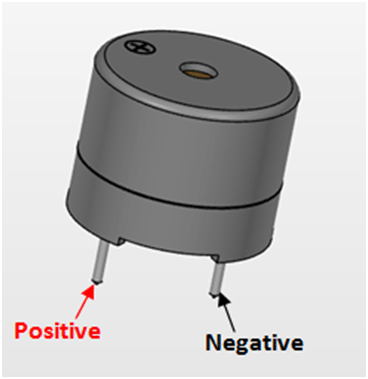
\includegraphics[scale=.5]{Buzzer-Pinout.png}
	\caption{Buzzer Pinout.}
\end{figure}
\subsection{Zero PCB Board}
Zero PCB is basically a general-purpose printed circuit board (PCB), also known as perfboard or DOT PCB. It is a thin rigid copper sheet with holes pre-drilled at standard intervals across a grid with 2.54mm (0.1-inch) spacing between holes. Each hole is encircled by a round or square copper pad so that component lead can be inserted into the hole and soldered around the pad without short-circuiting the nearby pads and other leads. For connecting the lead of component with another lead, solder these together or join these using a suitable conducting wire.
\begin{figure}[h]
	\centering
	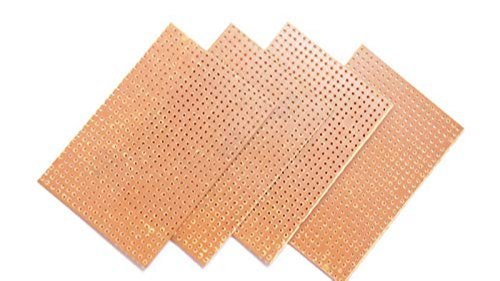
\includegraphics[scale=.5]{general-purpose-printed-circuit-board-mini-7-5-x-5-cm-mini-zero-pcb-board-500x500.jpg}
	\caption{Zero PCB Board.}
\end{figure}
\subsection{HT12D}
HT12D IC is a CMOS series 12-bit RF decoder. Mostly remote control applications have this technology. It gets to interface with the third device and helps it to decode 12-bits data. In this decoder, only 4-bits are data the remaining part is the address. The address will describe the location but 4-bits combination could make 16 types of different combinations. The HT12D decoder can not work alone. It works with another counterpart called an encoder. To receive the data between encoder and decoder address bits should be matched. The encoder can with any CMOS technology. Most modern applications use the encoder for decoding due to its simplicity and efficiency.\pagebreak
\begin{figure}[h]
	\centering
	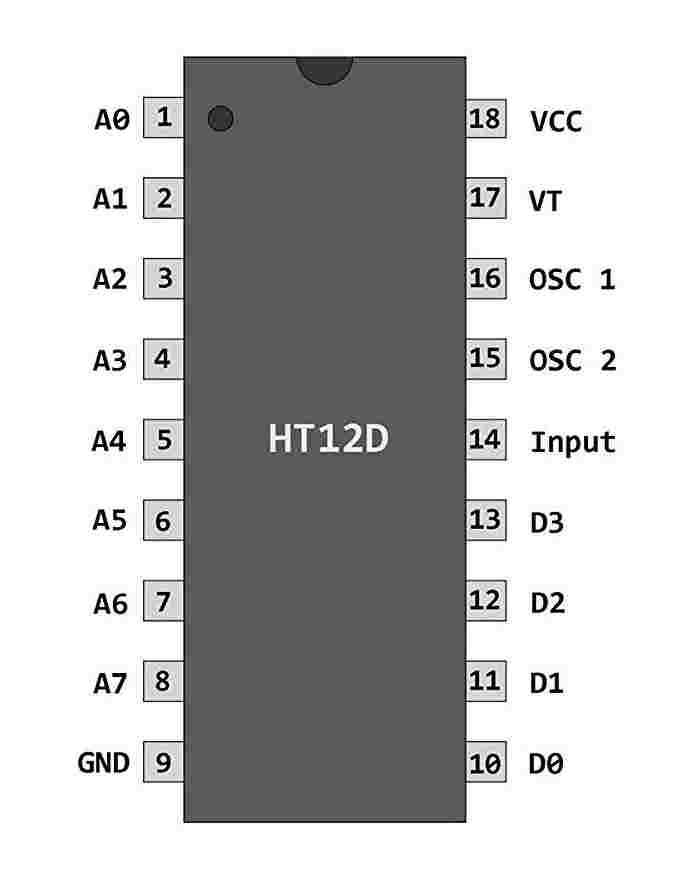
\includegraphics[scale=.3]{HT12D-pinout-diagram.jpg}
	\caption{HT12D Pinout Diagram.}
\end{figure}